\documentclass[english,9pt]{beamer}

\usepackage{amsmath} % load this before unicode-math
\usepackage{amssymb}
%\usepackage{unicode-math}

\usepackage{fontspec}
\setmonofont{DejaVu Sans Mono}
%\setmathfont{STIXMath}
%\setmathfont{TeX Gyre Termes Math}

\usefonttheme[onlymath]{serif}

\setlength{\parskip}{\smallskipamount}
\setlength{\parindent}{0pt}

\setbeamersize{text margin left=5pt, text margin right=5pt}

\usepackage{amsmath}
\usepackage{amssymb}
\usepackage{braket}

\usepackage{minted}
\newminted{julia}{breaklines,fontsize=\scriptsize,texcomments=true}
\newminted{python}{breaklines,fontsize=\scriptsize,texcomments=true}
\newminted{bash}{breaklines,fontsize=\scriptsize,texcomments=true}
\newminted{text}{breaklines,fontsize=\scriptsize,texcomments=true}

\newcommand{\txtinline}[1]{\mintinline[fontsize=\scriptsize]{text}{#1}}
\newcommand{\jlinline}[1]{\mintinline[fontsize=\scriptsize]{julia}{#1}}

\definecolor{mintedbg}{rgb}{0.95,0.95,0.95}
\usepackage{mdframed}

%\BeforeBeginEnvironment{minted}{\begin{mdframed}[backgroundcolor=mintedbg]}
%\AfterEndEnvironment{minted}{\end{mdframed}}

\setcounter{secnumdepth}{3}
\setcounter{tocdepth}{3}

\makeatletter

 \newcommand\makebeamertitle{\frame{\maketitle}}%
 % (ERT) argument for the TOC
 \AtBeginDocument{%
   \let\origtableofcontents=\tableofcontents
   \def\tableofcontents{\@ifnextchar[{\origtableofcontents}{\gobbletableofcontents}}
   \def\gobbletableofcontents#1{\origtableofcontents}
 }

\makeatother

\usepackage{babel}

\begin{document}


\title{\texttt{PWDFT.jl}: Density Functional Theory Calculations with Julia}
\subtitle{Introduction and Current Status}
\author{Fadjar Fathurrahman}
\institute{
Engineering Physics Department \\
Research Center for Nanoscience and Nanotechnology \\
Institut Teknologi Bandung
}
\date{24 September 2019}


\frame{\titlepage}

\section{Introduction}

\begin{frame}[plain]
\begin{center}
\Huge{Examples}
\end{center}
\end{frame}


\begin{frame}
\frametitle{Software packages for DFT calculations}

There are a lot of software packages for DFT calculations, for examples:
\begin{itemize}
\item Quantum ESPRESSO
\item VASP
\item ABINIT
\item Gaussian series: G03, G09, G16
\item NWchem
\end{itemize}

More extensive list:
{\scriptsize
\url{https://en.wikipedia.org/wiki/List_of_quantum_chemistry_and_solid-state_physics_software}
}

\end{frame}


\begin{frame}
\frametitle{Problems}

\begin{itemize}
\item These packages are very helpful for doing various calculations based on DFT.
%
These packages are suitable for black-box-type calculations where we are only concerned about the results.
%
\item However they are generally rather difficult to extend.
  \begin{itemize}
  \item New development on the DFT functionals:
  users generally need to wait for the next release of the package to use them
  (if these functionals are to be implemented at all).
  \item Custom calculations or post-processing steps:
  Users need to know in some detail
  about how the data they are interested in is represented or implemented in the package's source code.
  \end{itemize}
\end{itemize}

\end{frame}

\begin{frame}
\frametitle{Introducing PWDFT.jl}

\begin{itemize}
\item A package (more or less like a library, no executable) for electronic structure calculations
based on DFT.
\item Available at {\scriptsize\url{https://github.com/f-fathurrahman/PWDFT.jl}}
\item Using plane wave basis functions.
\item Implemented using Julia programming language.
\item My latest attempt to implement DFT softwares, previous attempts:
\begin{itemize}
  \item \txtinline{ffr-LFDFT}: {\scriptsize\url{https://github.com/f-fathurrahman/ffr-LFDFT}},
  using Lagrange basis functions, implemented in Fortran.
  \item \txtinline{ffr-PWDFT}: {\scriptsize\url{https://github.com/f-fathurrahman/ffr-PWDFT}}
  also using plane wave basis functions, implemented in Fortran.
\end{itemize}
\item Starting point is my Julia implementation of the code by Prof. Tomas Arias described in
his Practical DFT course. I extended the code to handle nonlocal pseudopotentials and
multiple k-points.
\item Taking many ideas from Quantum ESPRESSO, KSSOLV, ELK, etc.
\item No logo yet.
\end{itemize}

\end{frame}


\begin{frame}
\frametitle{Why I write another DFT package?}

Writing a DFT package from scratch is not the solution for all
problems.

[Rant mode ON]

Several questions appeared during my early days with DFT:
\begin{itemize}
\item Why my calculations are slow? What makes my calculations slow?
\item Is this slowness justified? How can I make it faster?
\item What are actually calculated by the DFT packages?
\end{itemize}

Learn by doing: how DFT or Kohn-Sham equations are solved (beyond
described in textbooks or research papers)

Frustation when trying to extend functionalities of available packages.

Educational purpose: the secret art of writing a DFT code is not yet documented
extensively in a book.

\end{frame}

\begin{frame}
\frametitle{Programming languages for DFT}
    
Programming languages used:
\begin{itemize}
\item Fortran and/or C/C++: ABINIT, VASP, Quantum Espresso, ...
\item Python: GPAW
\item MATLAB: KSSOLV, RESCU
\end{itemize}
    
Static languages: Fortran, C/C++

Dynamic languages: Python and MATLAB

\end{frame}



\begin{frame}
\frametitle{Julia programming language}

A rather new programming language (2012)

Syntax is familar to MATLAB or Python users

support for multidimensional array and linear algebra

Loop is fast!

\end{frame}


\begin{frame}
\frametitle{Aims of PWDFT.jl}

\begin{itemize}
\item Friendly-to-developers DFT package: enables quick implementation of various algorithms
\item educational purpose: simple yet powerful enough to carry out practical DFT calculations
for molecular and crystalline systems.
\end{itemize}

\end{frame}

\section{Introduction to Julia}

\begin{frame}[plain]
\begin{center}
\Huge{(Short) Introduction to Julia}
\end{center}
\end{frame}

%---------------------
\begin{frame}[fragile]
\frametitle{Julia installation}

I am assuming familiarity with command line.

Download Julia the current stable of Julia at
{\scriptsize\url{https://julialang.org/downloads}}
for your operating system.

Unpack the tarball. Usually after unpacking the tarball you should see a new directory
created: \txtinline{julia-1.x.x}, where \txtinline{1.x.x} is the version of Julia.

\begin{textcode}
julia-1.x.x/
├── bin
├── etc
├── include
├── lib
├── libexec
├── LICENSE.md
└── share
\end{textcode}

\end{frame}


%---------------------
\begin{frame}[fragile]
\frametitle{Julia installation (cont'd)}

The Julia binary resides within the \txtinline{bin} directory. You can launch Julia interpreter
by executing the \txtinline{bin/julia} executable. After executing the binary you can see the
the following output:
\begin{textcode}
                _
    _       _ _(_)_     |  Documentation: https://docs.julialang.org
   (_)     | (_) (_)    |
    _ _   _| |_  __ _   |  Type "?" for help, "]?" for Pkg help.
   | | | | | | |/ _` |  |
   | | |_| | | | (_| |  |  Version 1.3.1 (2019-12-30)
  _/ |\__'_|_|_|\__'_|  |  Official https://julialang.org/ release
 |__/                   |
 
 julia>
\end{textcode}

\end{frame}


%---------------------
\begin{frame}[fragile]
\frametitle{Install prerequisites}

\txtinline{PWDFT.jl} depends on several external packages:
\begin{itemize}
\item \txtinline{FFTW.jl}: used for Fast Fourier Transform (FFT).
\item \txtinline{SpecialFunctions}: used for evaluating special functions. For the moment
  this is used for evaluating error function.
\item \txtinline{LibSymspg.jl}: used for finding crystal symmetry and reducing k-points.
  This package is a Julia wrapper for \txtinline{spglib}
  {\scriptsize\url{https://github.com/atztogo/spglib}}.
\item \txtinline{Libxc.jl}: used for evaluating exchange-correlation energy and potential.
  This package is a Julia wrapper for Libxc {\scriptsize\url{https://gitlab.com/libxc/libxc}}.
\end{itemize}

The above packages can be installed by typing the following code in the Julia console.
You also need a working internet connection.
\begin{juliacode}
using Pkg
Pkg.add("FFTW")
Pkg.add("SpecialFunctions")
Pkg.add("LibSymspg")
Pkg.add("Libxc")
\end{juliacode}

\end{frame}



%---------------------
\begin{frame}[fragile]
\frametitle{Install PWDFT.jl}

PWDFT.jl is not yet a registered package so we need to use different command
to install it.
\begin{juliacode}
Pkg.add(PackageSpec(url="https://github.com/f-fathurrahman/PWDFT.jl"))
\end{juliacode}

Import the package by using:
\begin{juliacode}
using PWDFT
\end{juliacode}

It there is no error then we are ready to do some DFT calculations using
\txtinline{PWDFT.jl}.

\end{frame}


\begin{frame}[fragile]
\frametitle{Using Julia interactively}

Operators:

Variables:

Datatype:

Arrays:

Mathematical functions:

Functions:

LinearAlgebra:

\end{frame}


\begin{frame}
\frametitle{Typical steps}

Write Julia code not an input file.

Typical steps:
\begin{itemize}
\item Initialize Atoms
\item Initialize Hamiltonian with the given Atoms
\item Solve the Hamiltonian
\end{itemize}

Atomic units are used (energy: Hartree, length: bohr)

\end{frame}


\begin{frame}[fragile]
\frametitle{Example: hydrogen molecule in a box}

{\centering
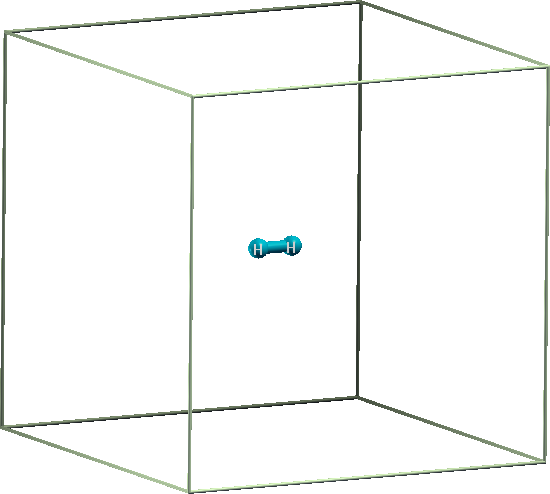
\includegraphics[width=0.25\textwidth]{codes/H2/H2.png}

}

\begin{juliacode}
using PWDFT # activate PWDFT package

# Initialize an H2 molecule in cubic box (simple cubic lattice)
# The coordinates are read from
atoms = Atoms( xyz_file="H2.xyz",
               LatVecs=gen_lattice_sc(16.0) )

pspfiles = ["H-q1.gth"] # pseudopotential parameters

ecutwfc = 15.0 # cutoff energy for wave function expansion

# initialize Hamiltonian
Ham = Hamiltonian( atoms, pspfiles, ecutwfc )

# solve the Kohn-Sham problem (using SCF algorithm)
KS_solve_SCF!( Ham )
\end{juliacode}


\end{frame}


\begin{frame}[fragile]
\frametitle{Output}

\begin{textcode}
$ julia run.jl 

Self-consistent iteration begins ...
update_psi = LOBPCG
mix_method = simple
Density mixing with betamix =    0.20000
    
-------------------------------------------------------
       iter            E            ΔE           Δρ
-------------------------------------------------------
SCF:     1      -0.9088890376  9.08889e-01  1.36287e-04
SCF:     2      -0.9197780666  1.08890e-02  1.17877e-04
SCF:     3      -0.9589404606  3.91624e-02  9.53668e-05
SCF:     4      -0.9975511159  3.86107e-02  7.60953e-05
.... # snipped
\end{textcode}

\end{frame}


\begin{frame}[fragile]
\frametitle{Converged Kohn-Sham energy components}

\begin{columns}[T]

\begin{column}{0.45\textwidth}
PWDFT.jl's result:
\begin{textcode}
-------------------------
Final Kohn-Sham energies:
-------------------------

Kinetic    energy:       1.0100082069
Ps_loc     energy:      -2.7127851088
Ps_nloc    energy:       0.0000000000
Hartree    energy:       0.9015229089
XC         energy:      -0.6314259148
PspCore    energy:      -0.0000012675
-------------------------------------
Electronic energy:      -1.4326811753
NN         energy:       0.3131700043
-------------------------------------
Total      energy:      -1.1195111709
\end{textcode}
\end{column}

\begin{column}{0.55\textwidth}

ABINIT's result:
\begin{textcode}
Components of total free energy (in Hartree) :

   Kinetic energy  =  1.01004059294567E+00
   Hartree energy  =  9.01545039301481E-01
   XC energy       = -6.31436384237843E-01
   Ewald energy    =  3.13170052325859E-01
   PspCore energy  = -1.26742500464741E-06
   Loc. psp. energy= -2.71283243086241E+00
   NL   psp  energy=  0.00000000000000E+00
   >>>>>>>>> Etotal= -1.11951439795224E+00
\end{textcode}
\end{column}

\end{columns}

\end{frame}

\begin{frame}
\frametitle{SCF solvers}

Kohn-Sham problem is solved using self-consistent field (SCF) iterations.
This is the most popular method.

In PWDFT.jl we can set various options to SCF algorithm:

\begin{itemize}
\item \jlinline{betamix}: linear mixing parameters (between 0 and 1)
\item \jlinline{mix_method}: linear, adaptive linear, Anderson, Pulay, restarted Pulay, periodic Pulay,
  and Broyden.
\item \jlinline{update_psi}: how to update the wave functions (iterative diagonalization or Chebyshev
subspace filtering).
\end{itemize}


\end{frame}

\begin{frame}
\frametitle{Direct energy minimization}

For systems with band gaps:

Conjugate gradient

Direct minimization

\end{frame}

\end{document}

